% Hikaru and Kelvin: final A selection. Never present a10 as part of this run.
\subsection{\expt{a112}: Full matched comparison}
\label{sec:a112-full}
We evaluated a112 as job 977773 against fresh baseline job 977740. Both ran
consecutively on xcnf0--4 using scale 1, seed 42, six client counts, 60-second
warmups, 600-second measurements and full logging. Data was reset between
client-count cases.

\begin{table}[htbp]
\caption{Matched baseline and a112 throughput; final failures remain visible.}
\label{tab:a-matched}
\begin{tabularx}{\linewidth}{@{}rRRRRR@{}}
\toprule
\textbf{Clients} & \textbf{a0 TPS} & \textbf{a112 TPS} & \textbf{Ratio} &
\shortstack{\textbf{a0 serial.}\\\textbf{failures}} &
\shortstack{\textbf{a112 serial.}\\\textbf{failures}} \\
\midrule
1 & 3.225 & 54.238 & $16.8\times$ & 0 & 0 \\
4 & 3.565 & 85.042 & $23.9\times$ & 0 & 0 \\
8 & 3.568 & 87.378 & $24.5\times$ & 2 & 0 \\
16 & 3.282 & 88.073 & $26.8\times$ & 20 & 0 \\
32 & 3.613 & 90.660 & $25.1\times$ & 64 & 0 \\
64 & 3.222 & 90.788 & $28.2\times$ & 59 & 0 \\
\bottomrule
\end{tabularx}
\end{table}

Both jobs completed every phase with exit code zero. A112 recorded no failed
measured transactions and passed all six post-run validation checks. The
unmodified a0 script has no post-run validation step. The baseline's failures
in Table~\ref{tab:a-matched} remain part of the interpretation: the ratios
describe achieved completed-script throughput under the recorded conditions.

\begin{table}[htbp]
\caption{A112 job 977773 latency (milliseconds) and retried transactions.}
\label{tab:a112-latency}
\begin{tabularx}{\linewidth}{@{}rRRRR@{}}
\toprule
\textbf{Clients} & \textbf{p50} & \textbf{p95} & \textbf{p99} &
\shortstack{\textbf{Retried}\\\textbf{transactions}} \\
\midrule
1 & 5.666 & 19.748 & 260.481 & 0 \\
4 & 9.423 & 313.624 & 814.970 & 0 \\
8 & 16.279 & 978.277 & 1,531.221 & 2 \\
16 & 23.309 & 2,407.638 & 3,101.652 & 2 \\
32 & 38.125 & 623.002 & 6,165.569 & 5 \\
64 & 63.958 & 6,597.911 & 10,030.710 & 16 \\
\bottomrule
\end{tabularx}
\end{table}

Every retried a112 transaction eventually succeeded. At 64 clients, p95 fell
from approximately 128,104\,ms in the matched baseline to 6,598\,ms, although
substantial tail latency remained. At one client, T3's mean fell from
2,656.9 to 6.8\,ms and T4's from 454.5 to 1.5\,ms, consistent with the intended
colocation benefit. The full comparison measures the combined design; it does
not assign the entire gain to an individual component.

\begin{figure}[htbp]
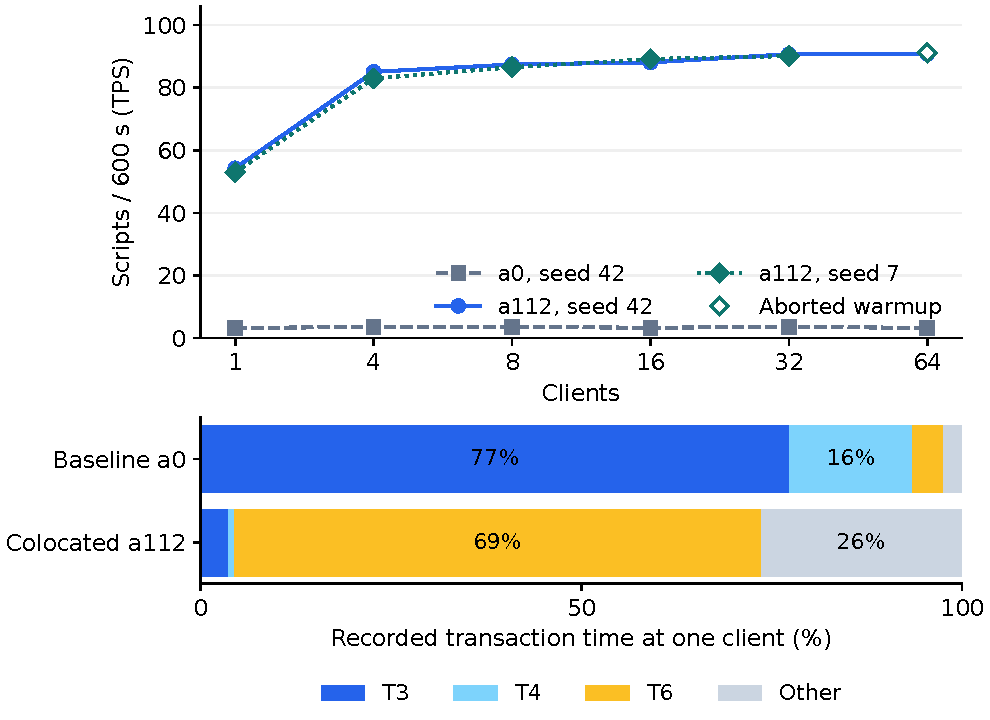
\includegraphics[width=\linewidth]{images/workload-a-full-matched.pdf}
\caption{Matched a0/a112 throughput and recorded transaction-time shares.
The open diamond flags the seed-7 repeat's aborted 64-client warmup.}
\label{fig:a-matched}
\end{figure}

The bottleneck shifted: T6 accounted for approximately 67--83\% of a112's
recorded transaction time, and throughput levelled off around 85--91 TPS from
four clients onward. More concurrency increased latency without proportional
throughput gains.

A seed-7 repeat, job 978177, produced measured TPS within 2.5\% of the seed-42
observations. Its 64-client warmup aborted, excluding that case from comparisons
requiring both phases to complete. Worker serialization cancellation was
reported as a Citus shard-commit error, which pgbench did not retry. The
repeat supports the observed performance while exposing an unresolved
concurrency limitation.
\evidence{\expt{a0}/job 977740; \expt{a112}/jobs 977773 and 978177.
Tables use \code{summary.csv}; the figure also uses \code{transaction_metrics.csv}.
Warmup and measurement exits were checked against the phase logs.}
